\documentclass[a4paper,12pt]{article}
\usepackage[notoc]{HaotianReport}
\usepackage{matlab-prettifier}
\headheight=14.0pt
\title{\SI{10}{\kW}光伏阵列建模及MPPT策略分析}
\author{邓思成,刘昊天}
\authorinfo{电41班, 2014010934, 2014010942}
\runninghead{太阳能光伏发电及其应用2017年最终报告}
\studytime{2017年6月}
\setmonofont{Consolas}
\lstMakeShortInline[style=Matlab-editor]"

\begin{document}
    \begin{abstract}
        最大功率点追踪(MPPT)是光伏系统并网发电的核心控制技术,一个高性能的MPPT系统可以显著提高光伏系统的发电能力。目前常规的MPPT算法有扰动观察(P\&O)法、电导增量法等,这些算法对于恒定光照单峰值的光伏电池具有良好的追踪性能。实际运行的光伏阵列的特性与理想光伏单元有差异,一是由于光照不均匀,光伏阵列的PV特性曲线通常会出现多峰值的现象,二是由于光照会发生变化,常规MPPT算法会出现误判现象。为解决这些问题,本文采用功率预测算法解决光照连续变化时常规算法的误判问题,并在此基础上提出了改进的全局定位算法,高效地解决了多峰值光伏阵列的最大功率点追踪问题。
        \begin{keywords}
            光伏发电,MPPT,多峰值,光照变化
        \end{keywords}
    \end{abstract}
    \maketitle
    %\newpage
    \section{实验目的} % (fold)
    \label{sec:实验目的}
    \begin{enumerate}[noitemsep, topsep=0pt]
        \item 检验课程学习结果
        \item 增强按目标寻找、归纳、组织知识点的能力
        \item 综合使用光伏发电相关知识
        \item 探索实际前沿问题的控制策略
    \end{enumerate}
    % section 实验目的 (end)
    \section{实验说明} % (fold)
    \label{sec:实验说明}
    任务见任务说明文档。

    在本次实验中,我们采用了MATLAB作为仿真平台,以m文件为基础,对各个任务进行了详尽的分析与解答。
    % section 实验说明 (end)
    \section{任务一} % (fold)
    \label{sec:任务一}
    \paragraph{任务描述} % (fold)
    本任务要求完成如下四点。
    % paragraph 任务描述 (end)
    \begin{enumerate}[noitemsep,topsep=0pt]
    \item 搭建光伏阵列模型,满足给定设置,能依据假定光照合理变化,能用于系统仿真;
    \item 实现 MPPT 控制策略,最经典的扰动观察和电导增量法中的一个即可;
    \item 实现改建的 MPPT 控制策略,可以使用变步长或者功率预测算法,也可以根据文献或者自己的想法给出的新策略;
    \item 对上述任务进行性能分析,包括光伏阵列特性曲线、MPPT 稳态特性、MPPT 暂态特性、改进 MPPT 性能提高对比分析等;
    \end{enumerate}

    \subsection{光伏阵列模型搭建} % (fold)
    \label{sub:光伏阵列模型搭建}
    我们知道,光伏阵列的UI特性可以表达为\cref{eq:iv}所示的公式与\cref{fig:pv}所示的电路。其中,$R_p$是一个并联大电阻,在本任务给定的条件下,其值很大,可以等效为$+\infty$。
    \begin{equation}
        I=I_{ph}-I_0\left(\exp{\left[\frac{q\left(U+I R_s\right)}{AKT}\right]}-1\right)-\frac{U+I R_s}{R_p}
        \label{eq:iv}
    \end{equation}
    \begin{figure}[htbp]
        \centering
        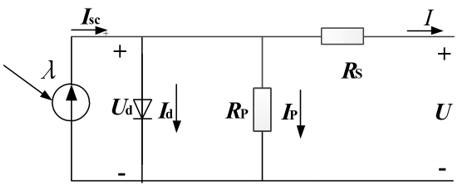
\includegraphics[width=0.65\textwidth]{pv.png}
        \caption{光伏板等效电路}
        \label{fig:pv}
    \end{figure}
    根据第二次作业中的推导,在给定$I_{sc},U_{oc},I_{mpp},U_{mpp},P_m=U_{mpp}I_{mpp}$的条件后,可以推导出“四参数”模型如\cref{eq:iv4,eq:Io,eq:Rs,eq:Iph,eq:N}所示。

    \begin{equation}
        I=I_{ph}-I_0\left(\exp{\left[\frac{U+I R_s}{N}\right]}-1\right)
        \label{eq:iv4}
    \end{equation}
    \begin{equation}\label{eq:Io}
          I_o=\displaystyle\frac{I_{ph}}{e^{CU_{oc}}-1}
    \end{equation}
    \begin{equation}\label{eq:Rs}
          R_s=\displaystyle\frac{1}{I_{mpp}}\left(U_{mpp}-\displaystyle\frac{I_{mpp}}{C\left(I_{ph}+I_o-I_{mpp}\right)}\right)
    \end{equation}
    \begin{equation}\label{eq:Iph}
          I_{ph}\approx I_{sc}
    \end{equation}
    \begin{equation}\label{eq:N}
          N=1/C\approx\displaystyle1/\left(\frac{1}{2U_{mpp}-U_{oc}}\left(\ln\displaystyle\frac{I_{ph}-I_{mpp}}{I_{ph}}+\displaystyle\frac{I_{mpp}}{I_{ph}-I_{mpp}}\right)\right)
    \end{equation}

    四参数模型中的$I_{ph}$是指在给定的测试条件下的光生电流,此处条件为\SI{1000}{\W\per\meter\squared}的光照强度。光生电流随温度、光照强度的变化情况如\cref{eq:iphlt}所示,其中$\alpha$为一常数。当温度不变时,有\cref{eq:iphlambda}所示的关系。在本任务中,可以以光生电流变化的比例反映光照强度变化的比例。
    \begin{equation}
        I_{ph}=I_{ph0}\left(1+\alpha \Delta T\right)\frac{\lambda}{1000}
        \label{eq:iphlt}
    \end{equation}
    \begin{equation}
        I_{ph} \propto \lambda, T=\text{const}
        \label{eq:iphlambda}
    \end{equation}

    在本任务中,逆变器看成一个理想的受控电压源,因此需要从光伏模型的$U$求解$I$。这需要求解一个非线性方程,使用MATLAB自带的fsolve函数求解较慢,因此采用朴素的牛顿迭代法求解,并排除不可行域($I>I_{ph}+I_0$)。这种方式使结果有实际意义,且提升了求解效率。单个光伏模型的代码如\cref{lst:single}所示。
    \lstinputlisting[label=lst:single,language=matlab]{../PvFunctionI.m}

    以上模型代码中增加了反并联二极管项,光伏单元端口电流中除\cref{fig:pv}中的光电流之外,还有反向并联的二极管电流,这一项电流在光伏单元正常工作的情况下可以忽略,光伏单元承受反压时将急剧增长。从实际意义上考虑,引入反并联二极管可以有效地避免光伏单元承受反压,在光伏单元串联而成的光伏阵列中具有实用价值。

    画出标准情况下的PV特性曲线和IV特性曲线,如\cref{fig:bare-pviv}所示。可以看到,其最大功率点、开路电压、短路电流与任务描述一致。
    \begin{figure}[htbp]
        \centering
        \includegraphics[width=0.8\textwidth]{../figure/bare-pviv.eps}
        \caption{原始光伏阵列特性曲线}
        \label{fig:bare-pviv}
    \end{figure}

    为了验证模型的正确性,可以令光照在\SIrange{100}{1200}{\W\per\meter\squared}范围内变化,观察其最大功率点的变化情况。可以看到\cref{fig:p-v-many}中,在这个合理的范围内,最大功率点组成的曲线是向右倾斜的,符合经验。
    \begin{figure}[htbp]
        \centering
        \includegraphics[width=0.8\textwidth]{../figure/p-v-many.eps}
        \caption{不同光照下的PV曲线}
        \label{fig:p-v-many}
    \end{figure}
    % subsection 光伏阵列模型搭建 (end)
    \subsection{常规MPPT控制策略} % (fold)
    \label{sub:常规mppt控制策略}
    最常见的MPPT控制策略有两种,即电导增量法INC和扰动观察法P\&O。本任务中,我们选择P\&O予以实现。根据经验,选择$0.9U_{oc}$作为起始点,执行跟踪算法。在我们的程序中,每个时刻代表的是动作的时刻,在其后的$dt$时间内(一般为\SI{0.1}{\s}),保持该状态不变。如\cref{fig:const-po,fig:const-po-upt}所示,在光照不变的条件下,该算法很好地跟踪了最大功率点。
    \begin{figure}[htbp]
        \centering
        \includegraphics[width=0.8\textwidth]{../figure/const-p&o.eps}
        \caption{P\&O在光照恒定条件下跟踪情况}
        \label{fig:const-po}
    \end{figure}
    \begin{figure}[htbp]
        \centering
        \includegraphics[width=0.8\textwidth]{../figure/const-p&o-upt.eps}
        \caption{P\&O在光照恒定条件下跟踪情况}
        \label{fig:const-po-upt}
    \end{figure}

    然而,当光照按照任务描述中发生变化时,该算法并不能很好地跟踪最大功率点,而出现错误的动作。如\cref{fig:po-fault,fig:po-fault-upt}所示,当光照降低时不会产生误判,而光照上升时,该算法无法跟踪最大功率点,功率曲线的形状较之光照曲线的形状发生了畸变。因此,还需要对P\&O进行改良。

    \begin{figure}[htbp]
        \centering
        \includegraphics[width=0.8\textwidth]{../figure/p&o-fault.eps}
        \caption{P\&O在光照变化下的跟踪情况}
        \label{fig:po-fault}
    \end{figure}
    \begin{figure}[htbp]
        \centering
        \includegraphics[width=0.8\textwidth]{../figure/p&o-upt-fault.eps}
        \caption{扰动观察法在光照变化下的电压、功率情况}
        \label{fig:po-fault-upt}
    \end{figure}
    % subsection 常规mppt控制策略 (end)
    \subsection{改进MPPT:功率预测法} % (fold)
    \label{sub:改进mppt_功率预测法}
    为解决光照发生变化时常规扰动观察法的误判问题,将常规P\&O算法改进为使用功率预测的P\&O法。功率预测法的基本思路如下:
    \begin{enumerate}
      \item 记两次电压控制时间间隔为$\Delta t$,$t=0$时进行一次电压控制,记录此时光伏阵列输出功率$P\left(0\right)$;
      \item $t=0.5\Delta t$时,测量光伏阵列输出功率$P\left(0.5\Delta t\right)$;
      \item $t=\Delta t$时的功率预测值$P'\left(\Delta t\right)=2P\left(0.5\Delta t\right)-P\left(0\right)$;
      \item $t=\Delta t$进行电压控制,记录输出功率$P\left(\Delta t\right)$,与$P'\left(\Delta t\right)$进行比较判断下次电压修正方向。
    \end{enumerate}
    使用功率预测法实现的MPPT追踪情况如\cref{fig:po,fig:po-upt}所示,可以看到,在光照不变、连续上升、连续下降的过程中,算法都能够对最大功率点进行较为有效的跟踪。
    \begin{figure}[htbp]
        \centering
        \includegraphics[width=0.8\textwidth]{../figure/p&o.eps}
        \caption{功率预测法在光照变化下的跟踪情况}
        \label{fig:po}
    \end{figure}
    \begin{figure}[htbp]
        \centering
        \includegraphics[width=0.8\textwidth]{../figure/p&o-upt.eps}
        \caption{功率预测法在光照变化下电压、功率情况}
        \label{fig:po-upt}
    \end{figure}
    % subsection 改进mppt_功率预测法 (end)
    \subsection{算法性能分析} % (fold)
    \label{sub:算法性能分析}
    通过光伏系统的MPPT效率来衡量MPPT算法的性能,MPPT效率通过\cref{eq:mppteff}定义。容易理解,MPPT算法性能越好,光伏系统就会具有更高的MPPT效率。
    \begin{equation}\label{eq:mppteff}
      \eta_{MPPT}=\frac{\text{光伏系统实际输出功率}}{\text{光伏系统当前光照、温度下能够输出的最大功率}}\times\SI{100}{\percent}
    \end{equation}
    \begin{figure}[htbp]
        \centering
        \includegraphics[width=0.8\textwidth]{../figure/mppt-eff.eps}
        \caption{功率预测法和常规P\&O法的MPPT效率比较}
        \label{fig:mppt-eff}
    \end{figure}
    
    \cref{fig:mppt-eff}绘制了给定光照变化情况下常规P\&O法和功率预测法的MPPT效率随时间变化曲线。可以看到,除了系统启动过程之外,功率预测法都具有更高的MPPT效率,而在系统启动时,由于功率预测法默认光伏阵列初始输出功率为0,导致第一次电压控制时判断失误,从而较常规P\&O法慢一个控制周期。对于持续运行的光伏系统,功率预测法的性能明显由于常规P\&O法,其劣势在于光伏阵列电压电流采样频率较高,对控制系统提出更高要求。

    % subsection 算法性能分析 (end)
    % section 任务一 (end)
    \section{任务二} % (fold)
    \label{sec:任务二}
    \paragraph{任务描述} % (fold)
    本任务要求完成如下三点。
    % paragraph 任务描述 (end)
    \begin{enumerate}[noitemsep,topsep=0pt]
    \item 将任务一中的光伏阵列分拆成具有串并联结构的几个子阵列,光照均匀时,总阵列的输出特性与任务一中的光伏阵列相同,合理设置子阵列的光照参数,使总阵列输出的 P-V 特性曲线上有两个(包含两个)以上的局域最大功率点,并且全局最大功率点电压和开路电压之间存在至少一个局域最大功率点,实现该光伏阵列模型。
    \item 保持光照不变,实现多峰值光伏阵列上的常规 MPPT 控制策略仿真和分析。
    \item 保持光照不变,尝试能够应对多峰值光伏阵列的新型 MPPT 控制策略,并给出分析。
    \end{enumerate}
    \subsection{多峰值光伏阵列} % (fold)
    \label{sub:多峰值光伏阵列}
    在\cref{sub:光伏阵列模型搭建}中实现的光伏单元模块的基础上,本任务使用4块光伏单元串并联连接实现多峰值光伏阵列,为避免光伏单元承受反压而降低能量输出效率,每一块光伏阵列均配有反并联二极管,如\cref{fig:pvarray}所示。4块光伏单元的光照强度可以独立变化,当其光照强度相差较大时,总阵列的输出特性将出现多峰值现象。
    \begin{figure}[htbp]
        \centering
        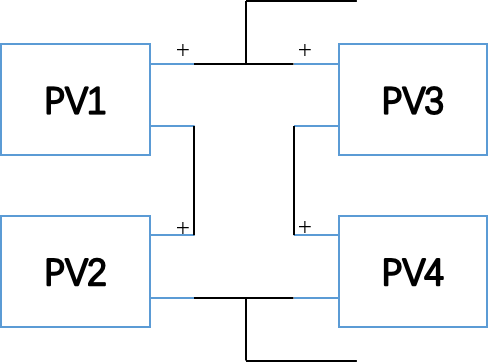
\includegraphics[width=0.7\textwidth]{pvarray.png}
        \caption{光伏阵列串并联结构}
        \label{fig:pvarray}
    \end{figure}

    考虑基于\cref{sub:光伏阵列模型搭建}中实现的光伏单元模型实现用于仿真的多峰值光伏阵列模型。光伏单元模型通过加压求流方式实现,数学上可看作函数$I=I\left(U\right)$。对于\cref{fig:pvarray}中的多峰值模型,4块光伏单元的模型可用$I_k=I_k\left(U_k\right)\ k\in\left\{1,2,3,4\right\}$描述,光伏阵列的电压、电流关系可用\cref{eq:pvarray}表示。
    \begin{equation}\label{eq:pvarray}
      \left\{
      \begin{aligned}
      I_1&=I_1\left(U_1\right) &I_2&=I_2\left(U_2\right)\\
      I_3&=I_3\left(U_3\right) &I_4&=I_4\left(U_4\right)\\
      I&=I_1+I_3=I_2+I_4 &I_1&=I_2\\
      U&=U_1+U_2 &U&=U_3+U_4
      \end{aligned}\right.
    \end{equation}

    整理\cref{eq:pvarray},得到简化后的\cref{eq:pvarraysim}。
    \begin{equation}\label{eq:pvarraysim}
      \left\{
      \begin{aligned}
      I&=I_1\left(U_1\right)+I_3\left(U_3\right)\\
      U&=I_1\left(U_1\right)+I_2\left(U-U_1\right)\\
      U&=I_3\left(U_3\right)+I_4\left(U-U_3\right)
      \end{aligned}\right.
    \end{equation}
    根据\cref{eq:pvarraysim}实现的4单元光伏阵列模型代码如\cref{lst:multi}所示。
    \lstinputlisting[label=lst:multi,language=matlab]{../Pv4SeriesParallel.m}
    各光伏单元光照强度如\cref{tbl:4Iph}所示,在给定光照设置下绘制光伏阵列的PV、IV特性曲线如\cref{fig:curve-multimax}所示。
    \begin{table}[htbp]
      \centering
      \setlength{\abovecaptionskip}{0pt}
      \setlength{\belowcaptionskip}{10pt}
      \caption{不均匀光照下各光伏单元光照强度}\label{tbl:4Iph}
      \begin{tabular}{|c|c|c|c|c|}
        \hline
        序号 & 1 & 2 & 3 & 4 \\
        \hline
        光照(\si{\watt\per\meter\squared}) & 1000 & 300 & 900 & 100 \\
        \hline
      \end{tabular}
    \end{table}
    \begin{figure}[htbp]
        \centering
        \includegraphics[width=0.8\textwidth]{../figure/curve-multimax.eps}
        \caption{多峰值光伏曲线}
        \label{fig:curve-multimax}
    \end{figure}

    设全部光伏单元的光照强度均为\SI{1000}{\watt\per\meter\squared},光伏阵列的的PV、IV特性曲线如\cref{fig:curve-singlemax}所示,可以看到,此时光伏阵列特性曲线与\cref{fig:bare-pviv}相同。
    \begin{figure}[htbp]
        \centering
        \includegraphics[width=0.8\textwidth]{../figure/curve-singlemax.eps}
        \caption{均匀光照下的串并联阵列特性曲线}
        \label{fig:curve-singlemax}
    \end{figure}
    % subsection 多峰值光伏阵列 (end)
    \subsection{常规MPPT策略在多峰值情况下的应用} % (fold)
    \label{sub:常规mppt策略在多峰值情况下的应用}
    将\cref{sub:改进mppt_功率预测法}提出的功率预测MPPT算法用于\cref{fig:curve-multimax}所示的多峰值光伏阵列。追踪轨迹和电压、功率变化情况如\cref{fig:mppt-fail-pv,fig:mppt-fail-upt}所示。
    \begin{figure}[htbp]
        \centering
        \includegraphics[width=0.8\textwidth]{../figure/mppt-fail-pv.eps}
        \caption{多峰值下常规MPPT策略的跟踪轨迹}
        \label{fig:mppt-fail-pv}
    \end{figure}
    \begin{figure}[htbp]
        \centering
        \includegraphics[width=0.8\textwidth]{../figure/mppt-fail-upt.eps}
        \caption{多峰值下常规MPPT策略的电压、功率情况}
        \label{fig:mppt-fail-upt}
    \end{figure}
    容易看到,由于功率预测法未考虑光伏阵列存在多个功率极值点的问题,容易追踪到光伏阵列功率的某个局部极值点而不能寻找到最大功率点。为应对多峰值的光伏阵列的最大功率点追踪问题,应当在功率预测法的基础上提出能够寻找到全局最优点的算法。
    % subsection 常规mppt策略在多峰值情况下的应用 (end)
    \subsection{改进MPPT策略:改良的全局定位算法} % (fold)
    \label{sub:改进mppt策略_改良的全局定位算法}
    对于多块光伏单元构成的具有多峰值PV特性的光伏阵列,一种简单而常用的最大功率点追踪思路是在针对单峰值阵列的MPPT算法基础上每隔一段时间进行一次电压的全局扫描,以扫描得到的最大功率电压为起点进行最大功率点追踪\cite{葛俊杰赵争鸣-521}。这种方法的优势在于实现简单且可靠性高,而缺点在于每隔一段时间就要进行电压的全局扫描,扫描过程中光伏阵列的MPPT效率较低。一种提高算法性能的思路是尽量缩短电压扫描过程占用的时间,同时跳过某些输出功率极低几乎不可能是最大功率电压的电压点。本节基于这种思路,提出了一种改进的全局定位算法,与传统的采取全局扫描的定位算法相比,改进算法具有更短的扫描时间以及扫描过程中更高的MPPT效率,有效地提升了MPPT算法的性能。

    首先考虑均匀光照光伏单元在不同光照条件下的PV曲线形态,绘制光伏单元光照强度在\SIrange{100}{1000}{\watt\per\meter\squared}之间变化时的PV曲线如\cref{fig:p-v-one}。观察曲线族可以发现,光照在相当大的范围内变动时,光伏单元的最大功率点电压只发生了较小的变化,本任务中使用的光伏单元最大功率点电压随光照的变化情况如\cref{fig:umpp-iph-one}所示。
    \begin{figure}[htbp]
        \centering
        \includegraphics[width=0.8\textwidth]{../figure/p-v-one.eps}
        \caption{标幺功率、标幺电压关系曲线}
        \label{fig:p-v-one}
    \end{figure}
    \begin{figure}[htbp]
        \centering
        \includegraphics[width=0.8\textwidth]{../figure/umpp-iph-one.eps}
        \caption{最大功率点标幺电压随光照变化情况}
        \label{fig:umpp-iph-one}
    \end{figure}

    通过\cref{fig:p-v-one,fig:umpp-iph-one}容易想到,全局定位算法通过电压扫描的方式寻找最大功率点时,不需对全电压范围进行扫描,只需扫描光伏阵列的特定电压范围即能以极大的概率寻找到最大功率点。对于本任务中分析的单峰值额定光照下开路电压为$U_{oc}$的光伏单元,其最大功率点电压以较大的概率出现在\numrange{0.6}{0.75}$U_{oc}$附近,在接下来的分析中,不失一般性,记$k_1=0.6$,$k_2=0.75$。

    对于每条串联支路由N块光伏单元组成的光伏阵列,大多数情况下其PV特性中最多出现N个极值点\cite{项丽王冰-520},每一个极值点一定对应某一块或多块光伏单元接近最大功率状态($U\in\left(k_1U_{oc},\ k_2U_{oc}\right)$),其余光伏单元处于反并联二极管导通状态或位于其自身最大功率点和开路点之间($U\in\left(k_1U_{oc},\ U_{oc}\right)$)。于是,光伏阵列最大功率点电压应满足\cref{eq:Urange}描述的电压关系。应当注意,\cref{eq:Urange}中的$U_{oc}$特指额定光照下光伏单元的开路电压,而$U_{mpp}$是任意光照下的最大功率点电压。
    \begin{equation}\label{eq:Urange}
      U_{mpp}\in\bigcup_{n=1}^{N}\left(k_1nU_{oc},\ k_2U_{oc}+\left(n-1\right)U_{oc}\right)
    \end{equation}

    在电压扫描环节,只对满足\cref{eq:Urange}的电压点进行测试,可以减小电压扫描的数目。另外,扫描环节的作用仅仅是大致确定最大功率点的位置,因此电压扫描和MPPT过程可使用不同的电压控制步长,记为$DU$、$dU$。本任务中,取$DU=\SI{10}{\volt}$、$dU=\SI{5}{\volt}$。

    于是,改进的全局定位算法流程如下:
    \begin{enumerate}
      \item 扫描电压点取$DU$的整数倍,在光伏阵列全电压范围内找出全部满足\cref{eq:Urange}的电压点,将这一电压序列存储;
      \item 按生成的电压序列进行电压扫描,记录扫描过程中功率最大的电压点$U_m$;
      \item 以上步的$U_m$为起点,按\cref{sub:改进mppt_功率预测法}的算法进行最大功率点追踪;
      \item 距上次扫描时间间隔达到某设定值$T$(本任务中取$T=\SI{100}{\second}$)后,重新启动电压扫描;
    \end{enumerate}
    \begin{figure}[htbp]
        \centering
        \includegraphics[width=0.8\textwidth]{../figure/mppt-pv.eps}
        \caption{改良算法的跟踪轨迹}
        \label{fig:mppt-pv}
    \end{figure}
    \begin{figure}[htbp]
        \centering
        \includegraphics[width=0.8\textwidth]{../figure/mppt-upt.eps}
        \caption{改良算法的电压、功率变化情况}
        \label{fig:mppt-upt}
    \end{figure}

    使用改进的全局定位算法对\cref{fig:curve-multimax}描述的多峰值光伏阵列进行最大功率点追踪,追踪轨迹和电压、电流随时间变化关系如\cref{fig:mppt-pv,fig:mppt-upt}所示。

    可以看到,改进的全局定位算法的电压扫描范围准确地包含了光伏阵列的全部功率极值点,在电压扫描结束后,逆变器能够准确追踪到光伏阵列的最大功率点附近并开始最大功率点追踪。每隔\SI{100}{\second},电压扫描便会重启一次,以应对光照变化时最大功率点从一个局部极值点变为另一个的情况。从\cref{fig:mppt-upt}可看到,每次电压扫描占用时间约\SI{1}{\second},光伏阵列大部分时间仍处于MPPT效率较高的追踪状态。
    % subsection 改进mppt策略_改良的全局定位算法 (end)
    
    \subsection{算法性能分析} % (fold)
    \label{sub:算法性能分析2}
    对于多峰值光伏阵列的最大功率点追踪,使用\cref{sub:改进mppt策略_改良的全局定位算法}提出的算法能够在绝大部分情况下实现准确的定位。本算法具有以下几个特点:
    \begin{itemize}
      \item 对于光照变化较缓慢的光伏系统,本算法能够实现长期有效的MPPT追踪;
      \item MPPT系统的效率主要受电压扫描周期、范围的影响,对于一般的光伏阵列,应实现测试其PV曲线,得到适合其工作的电压扫描范围,并针对实际情况合理设定电压扫描周期;
      \item 对于光照变化较快的情况,若最大功率点不在两个局部极值点之间发生跳跃,则本算法能够实现准确追踪;
      \item 若光照变化较快且最大功率点在不同局部极值点之间发生跳跃,则本算法可能发生误判,可通过提高电压扫描频率以改善性能。
    \end{itemize}
    % subsection 算法性能分析 (end)
    % section 任务二 (end)
    
    \section{结语} % (fold)
    \label{sec:结语}
    本文对常规P\&O法、功率预测法和改进的全局定位算法3种MPPT算法在不同运行状态的光伏系统上的追踪性能进行了分析。P\&O算法最为简单,对控制系统提出最低的要求,但只有对单峰值恒定光照的光伏系统能够体现出较为良好的性能;功率预测法比常规P\&O法稍复杂,能够处理光照连续变化时最大功率点的准确追踪,但不能应对多峰值光伏阵列全局最优点的追踪;改进的全局定位算法使用周期性的电压扫描实现了光伏阵列全局最优点的定位,并通过对光伏单元特性的分析缩小了电压扫描的规模,与传统的全局定位算法相比提升了MPPT效率。
    % section 结语 (end)
    
    \section{致谢} % (fold)
    \label{sec:致谢}
    本次实验历时3周,期间获得了来自各方的建议,实验的顺利完成离不开各方人士的帮助。在此特别感谢袁立强老师对MPPT算法和电压波形提出的修改建议,并感谢在实验过程中与我们进行讨论的同学们。
    % section 致谢 (end)
    
    \newpage
    \bibliography{report}
    \bibliographystyle{unsrt}

    \begin{appendix}
        \section{分工情况} % (fold)
        \label{sec:fengong}
        \paragraph{邓思成} % (fold)
        \label{par:邓思成}
        部分模型代码;部分MPPT代码;部分报告;部分PPT;

        总体工作量:50\%。
        % paragraph 邓思成 (end)
        \paragraph{刘昊天} % (fold)
        \label{par:刘昊天}
        部分模型代码;部分MPPT代码;部分报告;部分PPT;

        总体工作量:50\%。
        % paragraph 刘昊天 (end)

        \section{程序清单} % (fold)
        \label{sec:code}
        \begin{itemize}
          \item "calcPvParamters.m":从外特性参数计算四参数模型参数;
          \item "generateReport.m":主程序;
          \item "IphFunction.m":\cref{sub:常规mppt控制策略}中光照变化函数;
          \item "Pv4SeriesParallel.m":4单元光伏阵列模型;
          \item "PvFunctionI.m":光伏单元模型;
          \item "testManySingle.m":不同光照下光伏单元PV曲线;
          \item "testMPPT.m":多峰值光伏阵列改进算法追踪;
          \item "testMPPTdynamic.m":光照变化下功率预测法光伏单元追踪;
          \item "testMPPTdynamic_fault.m":光照变化下P\&O法光伏单元追踪;
          \item "testMPPTfail.m":功率预测法多峰值光伏阵列追踪;
          \item "testMultiMaxCurve.m":多峰值光伏阵列特性曲线绘制;
          \item "testPO.m":恒定光照下P\&O法光伏单元跟踪;
          \item "testRange.m":光伏单元不同光照下标幺PV曲线绘制;
          \item "testSingle.m":简单光伏单元特性曲线绘制;
          \item "testSingleMaxCurve.m":4单元光伏阵列在均匀光照下特性曲线绘制;
          \item "contrib/":包含过程中的尝试代码。
        \end{itemize}
    \end{appendix}
\iffalse
\begin{itemize}[noitemsep,topsep=0pt]
%no white space
\end{itemize}
\begin{enumerate}[label=\Roman{*}.,noitemsep,topsep=0pt]
%use upper case roman
\end{enumerate}
\begin{multicols}{2}
%two columns
\end{multicols}
\fi
\end{document} 